\section{Related Work}


\todo[inline]{add literature related to the research questions: on entity linking, de-duplication, on survival analysis}

\subsection{Evaluation of information systems}
Shannon and Weaver \cite{shannon_weaver} state that output of an IS can be defined at different levels, at the:
\begin{enumerate}
\item \textbf{technical level}: the accuracy and efficiency of the system.
\item \textbf{semantic level}: the success of information conveying the intended meaning.
\item \textbf{effectiveness level}: the effect of information on the receiver 
\end{enumerate}

This implies that factors contributing to a succesful IS could also be defined at different levels. DeLone and McLean\cite{delone_mclean:1, delone_mclean:2} have gathered many factors from literature and grouped them into six distinct but interdependent categories, see figure \ref{fig:success_model} below.

\begin{figure}[h]
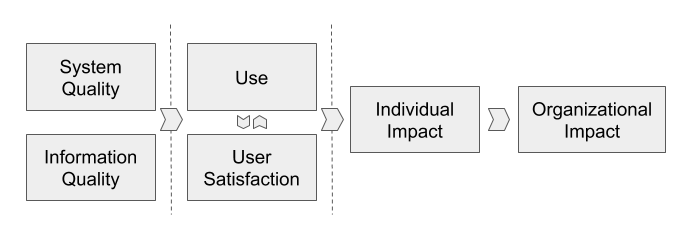
\includegraphics[width=1\linewidth]{images/dm_is_success_model.png}
\caption{DeLone and McLean Information Success Model.}
\label{fig:success_model}
\end{figure}

Each category or aspect of the I/S success measures still contains a number of variables that contribute to success:

\begin{itemize}
\item \textbf{System Quality}: measures the IS itself on the technical level. Example variables are data currency, completeness, and ease of use.
\item \textbf{Information Quality}: measures the IS output such as reports at the semantic level. Example variables are accuracy, precision and relevance.
\item \textbf{Information Use}: measures the actual use of the IS which is where the effectiveness level starts.
\item \textbf{User Satisfaction}: measures satisfaction from the perspective of the user, usually on an interval scale. This category is the mostly used as a single success measure and is fairly subjective.
\item \textbf{Individual Impact}: measures the information effect on the behaviour of the recipient.
\item \textbf{Organizational Impact}: measures the information effect on the performance of the organization.
\end{itemize}



\begin{comment}
	\subsection{Research Questions}
	The main research question is:
	\textbf{Is is possible to build a useful, complete and correct structured information system based on unstructured CIR data?}
	
	The system is build on three components
	\begin{itemize}
		\item extraction of insolvency process flow information.
		\item construction of a fully linked, clean entity structure of insolvents, administrators, judges, courts as well as administrator reports and court publications.
		\item extraction the text and parameters in administrator reports and indexes sections and parameters by imposing structure on the content.
	\end{itemize} 
	
	\begin{itemize}
		\item \textbf{useful}: the system is useful when it can answer questions of the parties involved or can answer these questions much more efficient than with current methods. We define so-called Persona to represent archetypical users of the information system and define specific questions they have. These questions are distilled from the insolvency law, news articles, research papers, court cases [refs] and interviews. [How do we measure, which section]
		\item \textbf{complete} the system's entity structure is complete when all main entities and their inter relations are found. Completeness is also defined for specific parameters needed to answer the user's questions. [How do we measure, which section]
		\item \textbf{accuracy} The system's identity structure is accurate when entities refer to their actual real life counterparts. The [How do we measure, which section]
	\end{itemize}
\end{comment}
